\documentclass[11pt]{article}
\usepackage[14pt]{extsizes}
%\usepackage[cp1251]{inputenc}
\usepackage[english,russian]{babel}
\usepackage{amssymb,latexsym,amsmath,euscript,amsfonts,amsthm}
\usepackage{color}
\linespread{1.5}

\usepackage{fontspec}
\usepackage{polyglossia}
\setdefaultlanguage{russian}
\setmainfont[Mapping=tex-text]{CMU Serif}
\usepackage[font=small]{caption}
\usepackage{subcaption}
\usepackage{hyperref}
\usepackage{sidecap}
\usepackage{float} %for fig position
\usepackage{graphicx}
\graphicspath{{pictures/}}
\DeclareGraphicsExtensions{.pdf,.png,.jpg}
\usepackage[left=30mm, top=20mm, right=30mm, bottom=20mm, nohead, footskip=10mm]{geometry}
%\setlength{\textfloatsep}{10pt plus 1.0pt minus 2.0pt}

\title{Курсовая работа}
\author{Соколова Ирина}

\newtheorem{theorem}{Теорема}
\newtheorem{lemma}{Лемма}
%\newtheorem*{corollary}{Следствие}[chapter]
\newtheorem{definition}{Определение}
%\newtheorem*{conjecture}{Гипотеза}
%\newtheorem*{example}{Пример}
%\newtheorem*{remark}{Замечание}[chapter]
%\newtheorem*{criteria}{Критерий}

\newcommand{\RomanNumeralCaps}[1]
    {\MakeUppercase{\romannumeral #1}}

%\newcounter{exercise}
%\newenvironment{exercise}{\refstepcounter{exercise}\smallskip\noindent\textbf{Упражнение~\theexercise.}}{}
%\numberwithin{exercise}

%\newenvironment{demo}{\noindent\textsl{Доказательство. }}{ $\square$ \medskip}

\begin{document}
\pagestyle{plain}
\makeatletter

\begin{titlepage}
\begin{center}
\textbf{Федеральное государственное автономное образовательное учреждение}\\
\textbf{высшего профессионального образования}\\
\textbf{"Национальный исследовательский университет}\\
\textbf{Высшая школа экономики"}\\
\textbf{Нижний Новгород}\\
\bigskip
\bigskip
\normalsize{Факультет Информатики,  Математики и Компьютерных Наук}\\
\normalsize{Программа подготовки бакалавров:}\\
\normalsize{ Фундаментальная математика}\\
\normalsize{ 2019-2020 учебный год}\\
%\bigskip
%\bigskip
%\bigskip
\bigskip
%\bigskip
\footnotesize\uppercase{курсовая работа}\\
\bigskip
\textbf{\large{О расположениях кубики и пары коник в}}\\
\textbf{\large{вещественной проективной плоскости}}\\
\end{center}
\bigskip
\bigskip
\bigskip
\begin{flushright}
\textbf{Выполнила:}\\
\normalsize{Соколова Ирина Максимовна}\\
\end{flushright}
\begin{flushleft}
\textbf{Научный руководитель:}\\
\normalsize{Кандидат физико-математических}\\
\normalsize{наук, доцент}\\
\normalsize{Полотовский Григорий Михайлович}\\
\normalsize{Подпись:}
\bigskip
\bigskip
\end{flushleft}
\vfill
\begin{center} Нижний Новгород, 2020 \end{center}
\end{titlepage}

\tableofcontents

\newpage
\section{Введение}


        На \RomanNumeralCaps{2} Международном Конгрессе математиков в Париже в 1900 году немецким математиком Д. Гильбертом были сформулированы 23 математические проблемы, которые предстояло решить в \RomanNumeralCaps{20} веке. Одной из этих проблем, а именно шестнадцатой, является «Проблема топологии алгебраических кривых и поверхностей». Шестнадцатая проблема Гильберта разбивается на две части, первая из которых – это исследование топологии неособых алгебраических кривых на проективной плоскости $\mathbb RP^2$ и неособых алгебраических поверхностей в проективном пространстве $\mathbb RP^3$. К теме шестнадцатой проблемы Гильберта примыкает задача исследования топологии вещественных алгебраических многообразий размерности $d$ в вещественном проективном пространстве $\mathbb RP^q$, где $q \geqslant 3, 1 \leqslant d \leqslant (q–1)$, а также исследование вещественных алгебраических многообразий с особенностями.
\newpage
\section{Постановка задачи}

\begin{definition}
 Плоской вещественной проективной алгебраической кривой степени m называется однородный многочлен $C_m(x_0, x_1, x_2)$ степени m с вещественными коэффициентами от трёх переменных $x_0, x_1, x_2$, рассматриваемый с точностью до ненулевого постоянного множителя.
\end{definition}

\begin{definition}
Множество $\mathbb RC_m$ точек вещественной проективной плоскости $\mathbb RP^2$ с координатами $(x_0:x_1:x_2)$, удовлетворяющими уравнению $C_m = 0$, называется множеством вещественных точек кривой $C_m$.
\end{definition}

\begin{definition}
Кривая $C_m$ называется неoсобой, если частные производные многочлена $C_m$ одновременно не равны нулю.
\end{definition}

\begin{definition}
Пусть $F$ -- однородный многочлен степени $m$ от переменных $x_1, x_2, x_3$. Если выполнено равенство $F = F_1 \cdot F_2$, где $F_1, F_2$ -- однородные многочлены степеней $m_1$ и $m_2$ соответственно, $1 \leqslant m_1 < m, 1 \leqslant m_2 < m$, то многочлен называется распадающимся, иначе -- нераспадающимся. Каждая из кривых $F_1 = 0$ и $F_2 = 0$ называется сомножителем кривой $F$.
\end{definition}

Каждая компонента связности множества  $\mathbb RC_m$ вещественных точек неособой кривой $C_m$ гомеоморфна окружности. В случае четной степени эта окружность называется овалом; каждый овал делит $\mathbb RP^2$ на две области: гомеоморфную диску и гомеоморфную листу Мебиуса. В случае нечетной степени среди вещественных ветвей кроме овалов имеется ровна одна ветвь, вложенная в $\mathbb RP^2$ односторонне, она называется нечетной ветвью.

\begin{theorem}[Теорема Харнака (1876)]
Пусть $N$ -- число вещественых ветвей кривой $C_m$. Тогда выполняется следующее неравенство $N \leqslant (m - 1) \cdot (m - 2)/2 + 1$, и эта оценка точна для любого $m$.
\end{theorem}

\begin{definition}
Кривые с максимально возможным по теореме Харнака числом ветвей называются М-кривыми.
\end{definition}

В этой работе мы будем рассматривать кривые степени 7, распадающиеся на две коники (обозначим их $C_2$ и $C_2^*$) и кубику (обозначим $C_3$) с выполнением следующих условий:

\begin{enumerate}
\item $C_3$, $C_2$, $C_2^*$ являются \textit{М}-кривыми.
\item Кривые, указанные в п. 1, попарно пересекаются без касания в максимально возможном (по теореме Безу) числе вещественных точек. Таким образом, $C_2$ и $C_3$ пересекаются в шести точках, $C_2^*$ и $C_3$ пересекаются в шести точках, $C_2$ и $C_2^*$ -- в  четырёх точках. 
\item Ни через какую точку не проходят сразу три кривые из п. 1.
\item Для каждой из коник $C_2$, $C_2^*$ по пять общих точек нечетной ветви кубики и коники лежат на одной из четырех внешних (то есть лежащих вне другой коники) дуг, на которые эта коника делится точками пересечения со второй коникой, а шестые точки пересечения лежат на одной из двух внутренних (то есть лежащих внутри другой коники) дуг.
\item Сначала нечетная ветвь пять раз пересекает первую конику, затем -- один раз вторую конику, затем -- первую конику один раз  и после пересекает вторую конику пять раз.
\end{enumerate}

Задача состоит в топологической классификации кривых такого вида в проективной плоскости. В этой работе мы выполним первый этап решения этой задачи: найдём список топологических моделей таких кривых, не противоречащих топологическим следствиям теоремы Безу.

\section{Перечисление допустимых моделей}
\begin{definition}
Назовём моделью расположения типа $1-5$ $($в дальнейшем -- просто модель$)$ набор четырёх топологических окружностей, ровно одна из которых вложена в $\mathbb RP^2$ односторонне и которая вместе с двумя из трёх остальных окружностей ведет себя с точки зрения числа и расположения общих точек так, как описано в пунктах $1-5$; четвёртая окружность не пересекается с первыми тремя.
\end{definition}

Будем учитывать известные сведения о взаимных расположениях \textit{М}-кубики и неособой коники \cite{litlink2}, \cite{litlink3}: имеются ровно три таких расположения, в которых нечётная ветвь кубики пересекает конику в шести вещественных точках (рисунок ниже).


\begin{figure}[H]
     \begin{subfigure}[b]{0.2\textwidth}
    \centering
    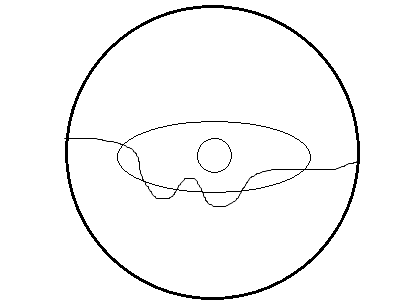
\includegraphics[scale=0.45]{loc_odd_brunch_1.png}
    \caption{}
  \end{subfigure}
  \hspace{2cm}
  \begin{subfigure}[b]{0.2\textwidth}
    \centering
    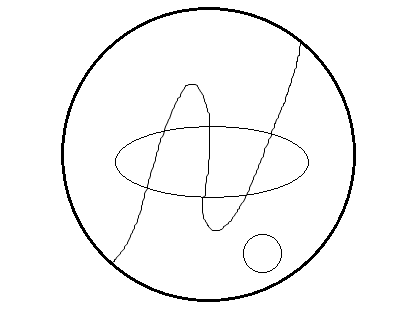
\includegraphics[scale=0.45]{loc_odd_brunch_2.png}
    \caption{}
  \end{subfigure}
  \hspace{2cm}
  \begin{subfigure}[b]{0.2\textwidth}
    \centering
    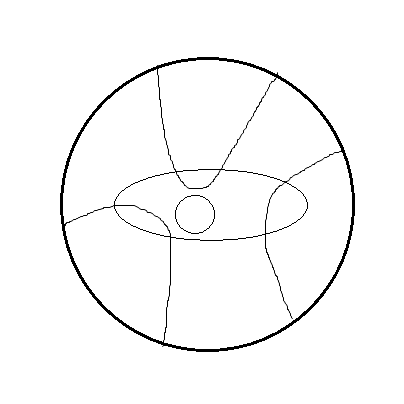
\includegraphics[scale=0.45]{loc_odd_brunch_3.png}
    \caption{}
  \end{subfigure}
\caption{Расположения нечетной ветви}
\label{fig:loc_odd_brunch}
\end{figure}

Третий случай пересечения коники нечетной ветвью в шести точках рассматриать не будем.

Пусть $\mathbb RC_2$ -- «горизонтальный» овал, $\mathbb RC_2^*$ -- «вертикальный» овал. Занумеруем точки, в которых нечётная ветвь пересекает эти овалы так, как показано на рисунке \ref{fig:model_1-5}. Рассмотрим все логически возможные способы прохождения нечётной ветви через эти 12 точек. Не нарушая общности, будем всегда рассматривать начало пересечения нечетной ветви с кониками на левой внешней дуге овала $\mathbb RC_2$. 

\begin{figure}[H]
\center{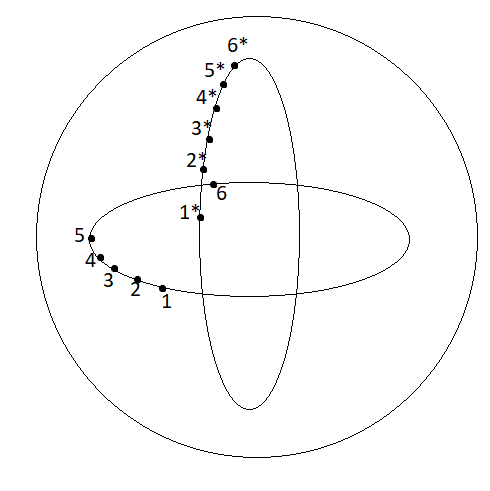
\includegraphics[scale=0.6]{model_1-5.png}}
\caption{Модель}
\label{fig:model_1-5}
\end{figure}

Будем записывать перестановку порядка 5 из номеров точек на вертикальной конике, получающуюся при движении вдоль нечётной ветви.  

Необходимо перебрать все перестановки степени 5. Большая часть перестановок запретится либо теоремой Безу (если провести прямую через точку, лежащую на левой внешней дуге горизонтального овала между точками 2 и 3 как на рисунке \ref{fig:two_bad_ex} (a), то она обязана будет пересечь нечётную ветвь кривой степени 3 в 5 точках), либо в силу того, что нечётная ветвь М-кривой не может иметь самопересечений (рисунок \ref{fig:two_bad_ex} (b)).



\begin{figure}[H]
     \begin{subfigure}[b]{0.2\textwidth}
    \centering
    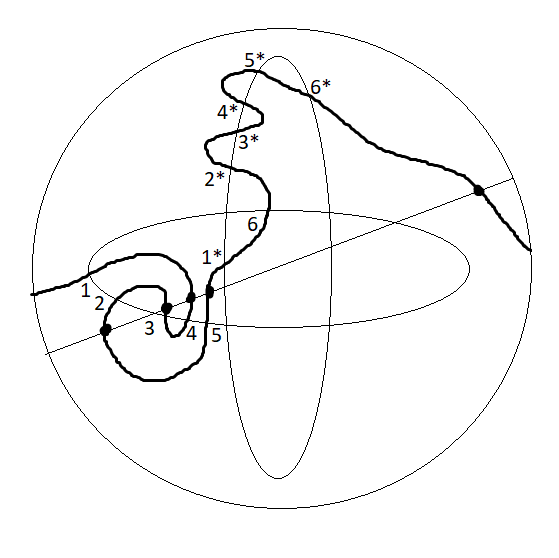
\includegraphics[scale=0.65]{two_bad_ex_1.png}
    \caption{}
  \end{subfigure}
  \hspace{4cm}
  \begin{subfigure}[b]{0.2\textwidth}
    \centering
    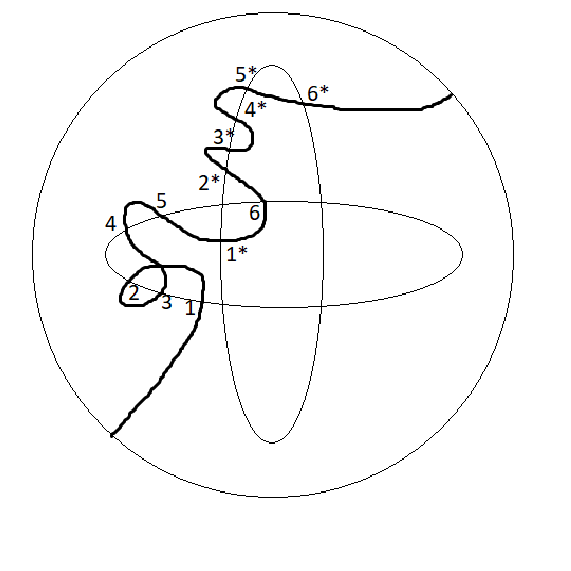
\includegraphics[scale=0.65]{two_bad_ex_2.png}
    \caption{}
  \end{subfigure}
\centering
\caption{}
\label{fig:two_bad_ex}
\end{figure}

Непосредственным перебором мы получим следующие возможные перестановки:\\
(54321), (54123) – (отвечает случаю (а) рис. \ref{fig:loc_odd_brunch})\\ 
(32145), (12345) – (отвечает случаю (b) рис. \ref{fig:loc_odd_brunch})\\

Существует два топологически различных расположения в $\mathbb RP^2$ двух неособых коник с четырьмя общими точками (рис. \ref{fig:intersection_of_ovals}).

\begin{figure}[H]
\center{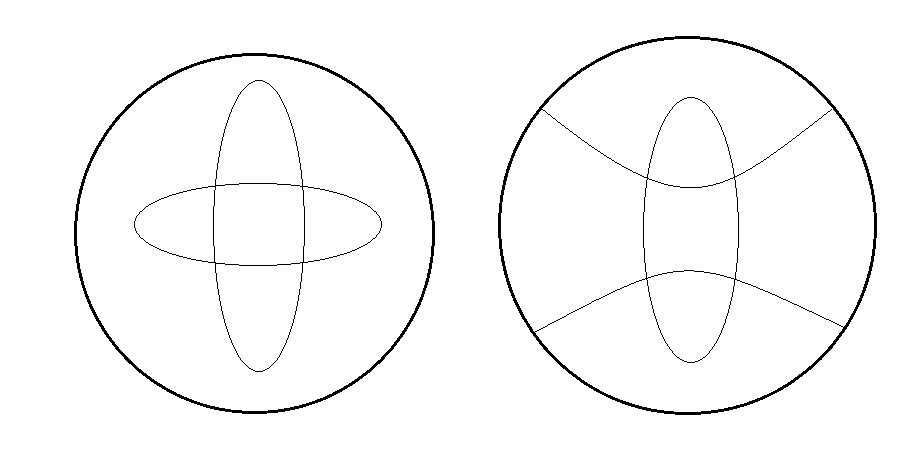
\includegraphics[scale=0.5]{intersection_of_ovals.png}}
\caption{}
\label{fig:intersection_of_ovals}
\end{figure}

Но в случае, который представлен на рисунке \ref{fig:intersection_of_ovals} справа, расположение нечетной ветви будет противоречить пункту 5 -- при соблюдении условий 1-4 не будет соблюдаться условие 5 (рис. \ref{fig:prohibit_second_inters_ovals}),  поэтому мы будем рассматривать только первый случай .

\begin{figure}[H]
\center{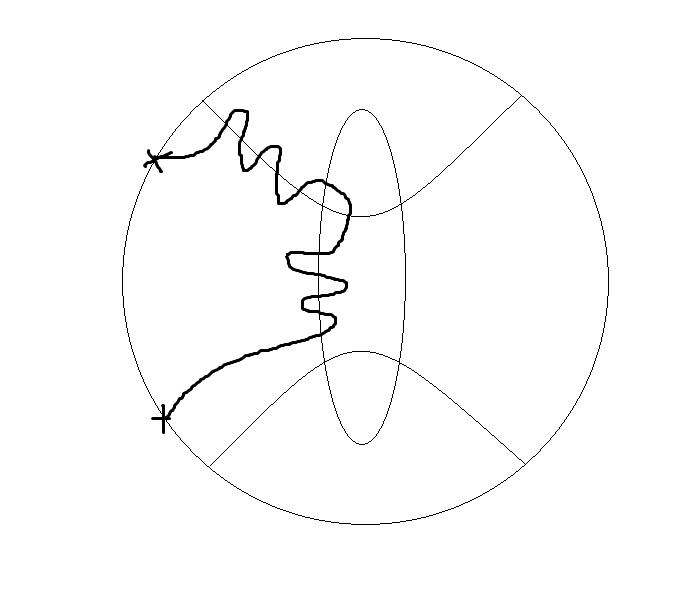
\includegraphics[scale=0.9]{prohibit_second_inters_ovals.png}}
\caption{}
\label{fig:prohibit_second_inters_ovals}
\end{figure}


Проиллюстрируем случаи пересечения нечетной ветви с кониками, соответствующие оставшимся подстановкам. Всего получится $4 \cdot 4 = 16$ иллюстраций, но некоторые из них дают гомеоморфные картинки, попарно негомеоморфных получилось 11. 

\begin{figure}[H]
\center{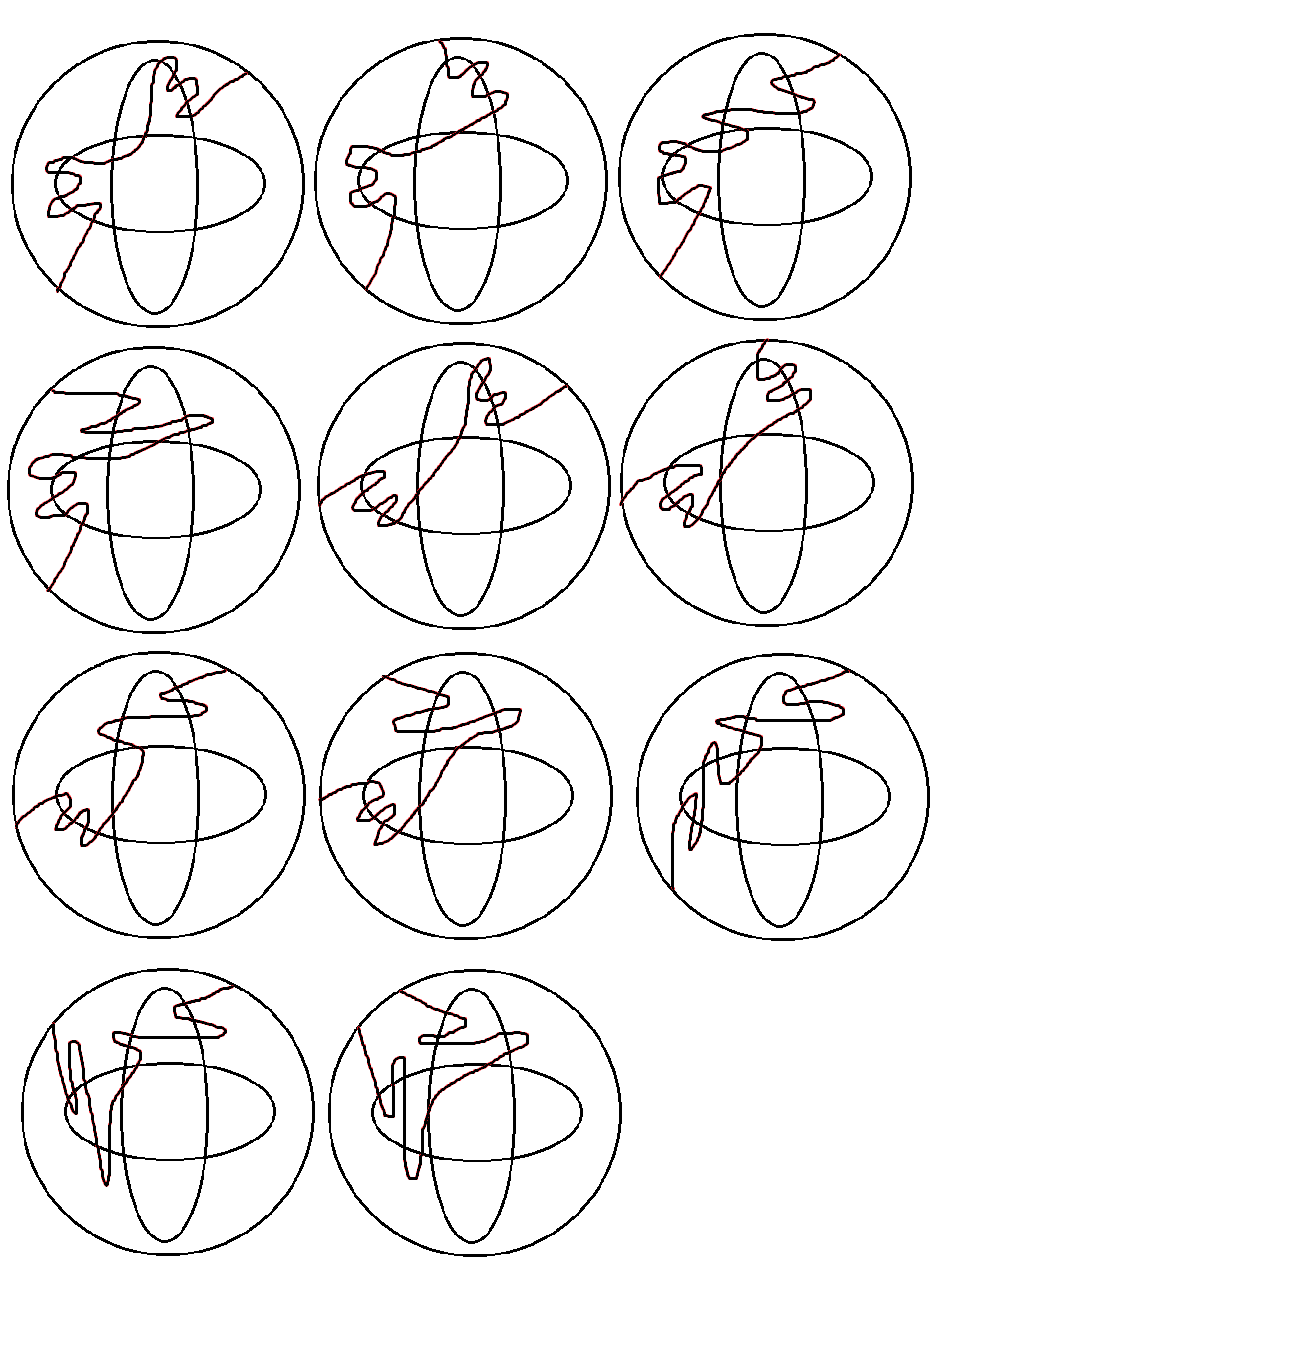
\includegraphics[scale=0.93]{curves_without_ovals.png}}
\caption{Модели без овала кубики}
\label{fig:curves_without_ovals}
\end{figure}

Допустимые для расположения овала кубики компоненты дополнения $\mathbb RP^2$ к объединению коники и кубики показаны на рисунке \ref{fig:loc_odd_brunch}.

Так как необходимо учитывать эти ограничения для каждой из двух коник, то для каждой ситуации (картинки) на рисунке \ref{fig:curves_without_ovals} надо найти пересечение допустимой области относительно одной коники с допустимой областью относительно второй коники. На рисунке \ref{fig:intersection_of_fields} показано пересечение областей, допустимых для овала, у первой модели на рисунке \ref{fig:curves_without_ovals}.

\begin{figure}[H]
\center{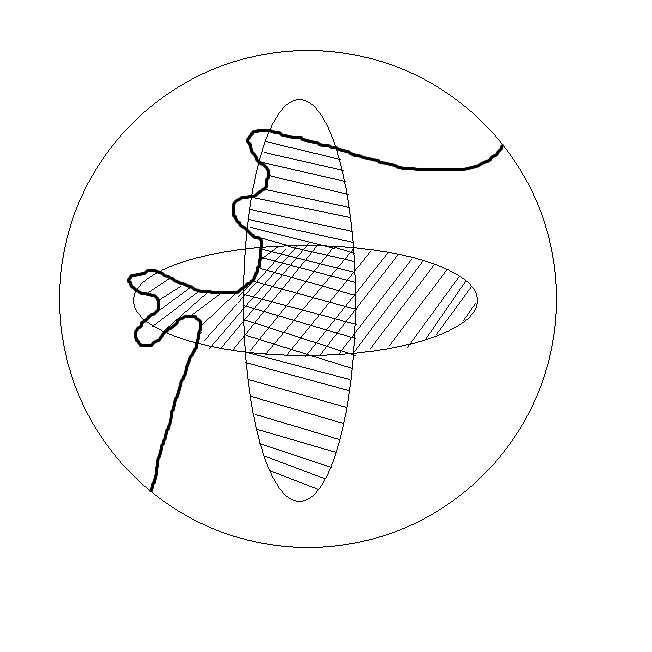
\includegraphics[scale=0.8]{intersection_of_fields.png}}
\caption{}
\label{fig:intersection_of_fields}
\end{figure}

Получим следующие возможные случаи:

\begin{figure}[H]
\center{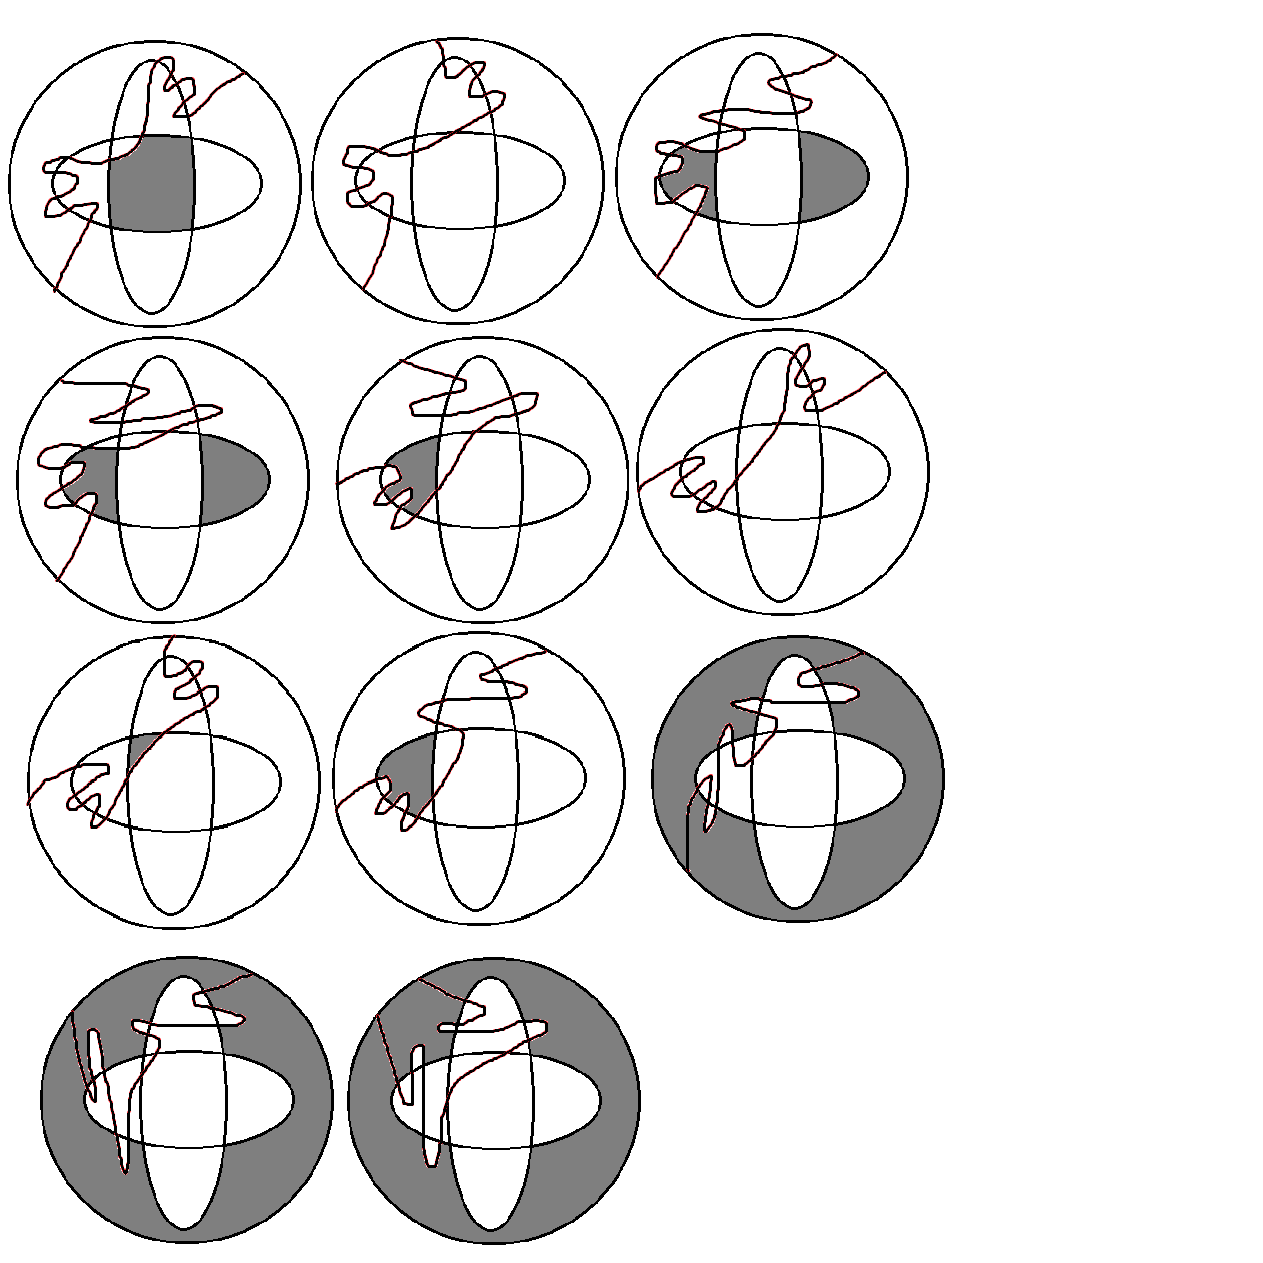
\includegraphics[scale=0.9]{curves_with_ovals.png}}
\caption{Модели с допустимыми областями для овала}
\label{fig:curves_with_ovals}
\end{figure}

Таким образом, 11 моделей подлежат дальнейшему исследованию на предмет реализуемости их алгебраическими кривыми рассматриваемого класса.

\newpage
\section{Заключение}
В данной курсовой работе мы доказали, что имеются четырнадцать попарно различных моделей кривых степени 7 рассматриваемого вида, допустимых топологическими следствиями теоремы Безу и некоторыми другими известными запретами. Дальнейшие этапы решения задачи -- применение для запретов метода Оревкова и некоторые построения -- будут рассмотрены в следующей работе.

\newpage
\addcontentsline{toc}{section}{Список используемой литературы}
\begin{thebibliography}{}
\bibitem{litlink1}{PA} Д. А. Гудков, Е. И. Шустин, Г. М. Полотовский "Топология вещественных алгебраических многообразий", г. Горький, издание ГТУ, 1986г.
\bibitem{litlink2}Полотовский Г. М. Топологическая классификация распадающихся кривых 6-го порядка // Дисс. на соиск. степ. канд. ф-м наук, Горький, 1979. 261 с

\bibitem{litlink3}Kuzmenko T., Polotovsky G. Classification of curves of degree 6 decomposing into a product of M-curves in general position // AMS Translations, Ser. 2, Vol. 173 "Topology of real algebraic Vsrieties and Related Topics". 1996.P.165-177

\end{thebibliography}


%%\@input{preface}
%%\@input{ch1_1}
%%\@input{bibliography}
\makeatother
\end{document}
